\begin{figure}[H]
    \centering
    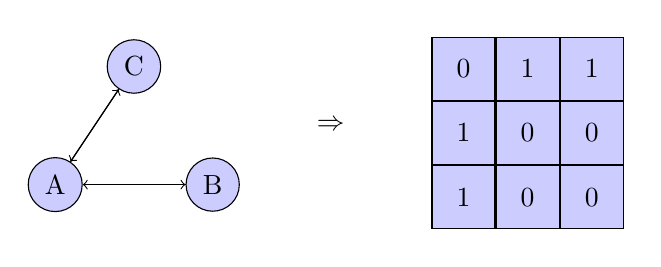
\begin{tikzpicture}
        \node[circle, draw, fill=blue!20] (A) at (0,0) {A};
        \node[circle, draw, fill=blue!20] (B) at (2,0) {B};
        \node[circle, draw, fill=blue!20] (C) at (1,1.5) {C};
        \draw[->] (A) -- (B);
        \draw[->] (A) -- (C);
        \draw[->] (B) -- (A);
        \draw[->] (C) -- (A);
        \node (RA) at (3.5,0.75) {$\Rightarrow$};
        \matrix (A) [nodes={draw, minimum size=0.8cm, fill=blue!20}, right=6cm, below=-2cm] {
            \node{0}; & \node{1}; & \node{1}; \\
            \node{1}; & \node{0}; & \node{0}; \\
            \node{1}; & \node{0}; & \node{0}; \\
        };
    \end{tikzpicture}
    \caption{Adjacency Matrix representation.}
    \label{fig:adjacency-matrix}
\end{figure}